\documentclass{article}%
\usepackage[T1]{fontenc}%
\usepackage[utf8]{inputenc}%
\usepackage{lmodern}%
\usepackage{textcomp}%
\usepackage{lastpage}%
\usepackage{authblk}%
\usepackage{graphicx}%
%
\title{c{-}Secretase inhibitor I induces apoptosis in chronic lymphocytic leukemia cells by proteasome inhibition, endoplasmic reticulum stress increase and Notch down{-}regulation}%
\author{Rebecca Benitez}%
\affil{Institute of Bioinformatics and Biosignal Transduction, College of Bioscience and Biotechnology, National Cheng{-}Kung University, Tainan, Taiwan}%
\date{01{-}01{-}2013}%
%
\begin{document}%
\normalsize%
\maketitle%
\section{Abstract}%
\label{sec:Abstract}%
Scientists found that curcumin prevented respiratory inflammation in mice. We originally developed curcumin as a disease modifier from the pharmacy of Rand McNally. The molecule is also used as an ingredient in Ayurvedic skin care. Curcumin is a turmeric derivative that works in a similar way to certain substances found in the fight against bronchiolitis.\newline%
Researchers at UC San Diego,the La Jolla Institute for Biomedical Research, and the University of North Carolina carried out the experiments while conducting ongoing work on infiltrating the immune system with probiotics or simple probiotic antibiotics. This is their first study to look into the behavior of nasal flora when the immune system is attacked by an invading disease.\newline%
Researchers discovered that curcumin reduced the chronic inflammation that takes place in the body when pathogens are present. As microbial invaders are attracted to a healthy mucosal barrier, they are effectively neutralized by curcumin.\newline%
According to UC San Diego, the behavior of the chronic inflammation in crows that discovered the inflammation{-}promoting effect of curcumin are differentiated from that of crows that detect invading pathogens. The researchers believe that these two different behaviors signal different immune response mechanisms in host.\newline%
Curcumin is used in a number of medicines in addition to healthful skin care products. The molecules have demonstrated significant efficacy against several gastrointestinal and metabolic disorders, including irritable bowel syndrome and lupus. Currently, curcumin is commonly used to treat sinusitis and irritable bowel syndrome.

%
\subsection{Image Analysis}%
\label{subsec:ImageAnalysis}%


\begin{figure}[h!]%
\centering%
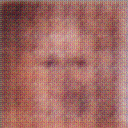
\includegraphics[width=150px]{500_fake_images/samples_5_486.png}%
\caption{A Close Up Of A Person With A Camera}%
\end{figure}

%
\end{document}